\chapter{Эволюция шланговой турбулентности магнитоактивной анизотропной плазмы}
\label{ch:ch4}
\section{Введение}\label{ch:ch4/sec1}

Развитие магнитной турбулентности в помещенной во внешнее однородное магнитное поле $\vec{B}_{ext}=(0, 0, B_{ext})$ бесстолкновительной плазме на временах, допускающих пренебрежение движением тяжелых ионов, описывается известными уравнениями Максвелла--Власова~\cite{Vlasov1967,Kocharovsky2016}. 
В данном случае они принимают следующий вид, аналогичный системе (\ref{eq:maxw1})-(\ref{eq:Vlasov}), для электрического $\vec{E}(\vec{r}, t)$ и магнитного $\vec{B}(\vec{r}, t)$ полей и функции распределения электронов $f(\vec{v},\vec{r}, t)$, зависящих от времени $t$, радиуса-вектора $\vec{r}=\left(x,y,z\right)$ и скорости $\vec{v}=\left(v_x,v_y,v_z\right)$
\begin{align}
     \label{eq:maxw1_b0} 
    \nabla \times \vec{B}=\dfrac{1}{c}\dfrac{\partial \vec{E}}{\partial t}+\dfrac{4\pi}{c}\vec{j}, \\
    %
    \label{eq:maxw2_b0}
    \nabla \times \vec{E}=-\dfrac{1}{c}\dfrac{\partial \vec{B}}{\partial t}, \\
    %
    \dfrac{\partial f}{\partial t}+\vec{v}\dfrac{\partial f}{\partial \vec{r}}-\dfrac{e}{\me} \left(\vec{E}+\dfrac{1}{c}\left[\vec{v},\vec{B}+\vec{B}_{ext}\right]\right) \dfrac{\partial f}{\partial \vec{v}}=0,
    \label{eq:Vlasov_b0}
\end{align}
где $c$~-- скорость света в вакууме, $e$ и $\me$~-- величина заряда и масса электрона, $\vec{j}=-e\iiint^{+\infty}_{-\infty}\vec{v}f(\vec{v},\vec{r}, t) d^3\vec{v}$~-- плотность тока, $N=\iiint^{+\infty}_{-\infty}f(\vec{v},\vec{r}, t) d^3\vec{v}$~-- концентрация электронов, $N_0$~-- ее начальное однородное значение. 
Для определенности вновь полагается, что в начальный момент времени нормированная функция распределения электронов по скоростям $\Psi = c^3f/N_0$ имеет бимаксвелловскую форму, вытянутую вдоль оси $z$, т.е. вдоль внешнего магнитного поля:
\begin{equation}
\label{eq:bimax_b0}
\Psi(\vec{\beta})=\dfrac{1}{\pi^{3/2}\beta_{\perp 0}^2 \beta_{\| 0} } \exp\left(-\dfrac{\beta_x^2+\beta_y^2}{\beta_{\perp 0}^2}-\dfrac{\beta_z^2}{\beta_{\| 0}^2}\right).
\end{equation}
Внешнее поле $B_{ext}$ будем предполагать относительно слабым, так что продольный бета-параметр больше или порядка единицы: $\frac{8\pi k_bNT_\|}{B_{ext}^2}\gtrsim1$, $k_b$ - постоянная Больцмана. 
Кинетическое моделирование и анализ свойств турбулентности подобной магнитоактивной плазмы актуален как для астрофизических задач, например, касающихся физики областей формирования солнечного (звездного) ветра и магнитосфер звезд и планет, так и для задач физики лабораторной плазмы, например, лазерной, получаемой при абляции мишени или струи газа фемтосекундными импульсами~\cite{Yoo2014,Park2012}.

Ключевыми параметрами в рассматриваемой начальной задаче о магнитной турбулентности являются начальная анизотропия $A_0$ распределения электронов по скоростям и нормированное внешнее магнитное поле $b_{ext}=B_{ext}/\sqrt{8\pi N T_{\|0}}\lesssim1$, равное обратному квадратному корню из плазменного бета-параметра. 
Данные величины не только задают диапазон первоначально неустойчивых мод, но и определяют дальнейшую нелинейную эволюцию спектра. 
Как уже говорилось ранее, дисперсионный анализ апериодической неустойчивости вейбелевского типа в анизотропной плазме без внешнего магнитного поля проведён весьма подробно~\cite{Weibel1959,Zhou2022,Fried1959,Kalman1968,Morse1971,Kocharovsky2016,Lazar2006,Stockem2009,SchaeferRolffs2006}. 
Этой неустойчивости подвержены исключительно TM-моды~\cite{Vagin2014}, т.е. моды, магнитное поле которых ортогонально плоскости, определяемой их волновым вектором и осью анизотропии бимаксвелловской плазмы~ (рис.~\ref{fig:TMmodes}). 
Наибольший линейный инкремент наблюдается у мод с волновым вектором, перпендикулярным к оси анизотропии, т.е. лежащим в плоскости $xy$, и поэтому называемых поперечными; для них диапазон неустойчивости включает волновые числа в промежутке $\left(0;\sqrt{A_0}\right)$ (см. главы \ref{ch:ch1} и \ref{ch:ch2}). 
По мере уменьшения угла $\theta$ между волновым вектором и осью анизотропии, инкремент ТМ-мод, теперь уже наклонных, довольно быстро спадает до нуля~\cite{Vagin2014}. 
\begin{figure}[h]
\includegraphics[width=0.35\linewidth]{part4/TMmodes.png}
\captionstyle{normal}
\centering
\caption{Взаимное расположение волнового вектора $\vec{k}$, лежащего в плоскости $x,z$, и векторов магнитного $\vec{B}$ и электрического $\vec{E}$ полей в отдельной пространственной моде ТМ-вейбелевской турбулентности.}
\label{fig:TMmodes}
\end{figure}
В присутствии внешнего однородного магнитного поля выделяют две ветви шланговых мод, отвечающие электронным так называемым "периодической" и "апериодической" шланговым неустойчивостям. 
Первая ветвь неустойчивости имеет место для волновых векторов, направленных преимущественно вдоль оси анизотропии, и инкремент таких мод много меньше их частоты, а область параметров, в которой неустойчивость развивается, является сравнительно узкой. 
Поэтому ей в настоящей главе уделено немного внимания. 
Другая ветвь шланговой неустойчивости, развивающаяся значительно быстрее, реализуется в более обширной области параметров и под б\'{о}льшими углами к оси анизотропии ~\cite{Li2000,Camporeale2008,Lazar2013,Shaaban2019,Moya2022}. 
Анализ дисперсионного соотношения показывает, что в общем случае моды этой ветви являются смешанными (не ТМ и не ТЕ), хотя при стремлении величины внешнего поля  к нулю, $B_{ext}\rightarrow0$, эта ветвь является ничем иным как дисперсионной ветвью апериодически неустойчивых вейбелевских ТМ-мод. 


\begin{figure}[h]
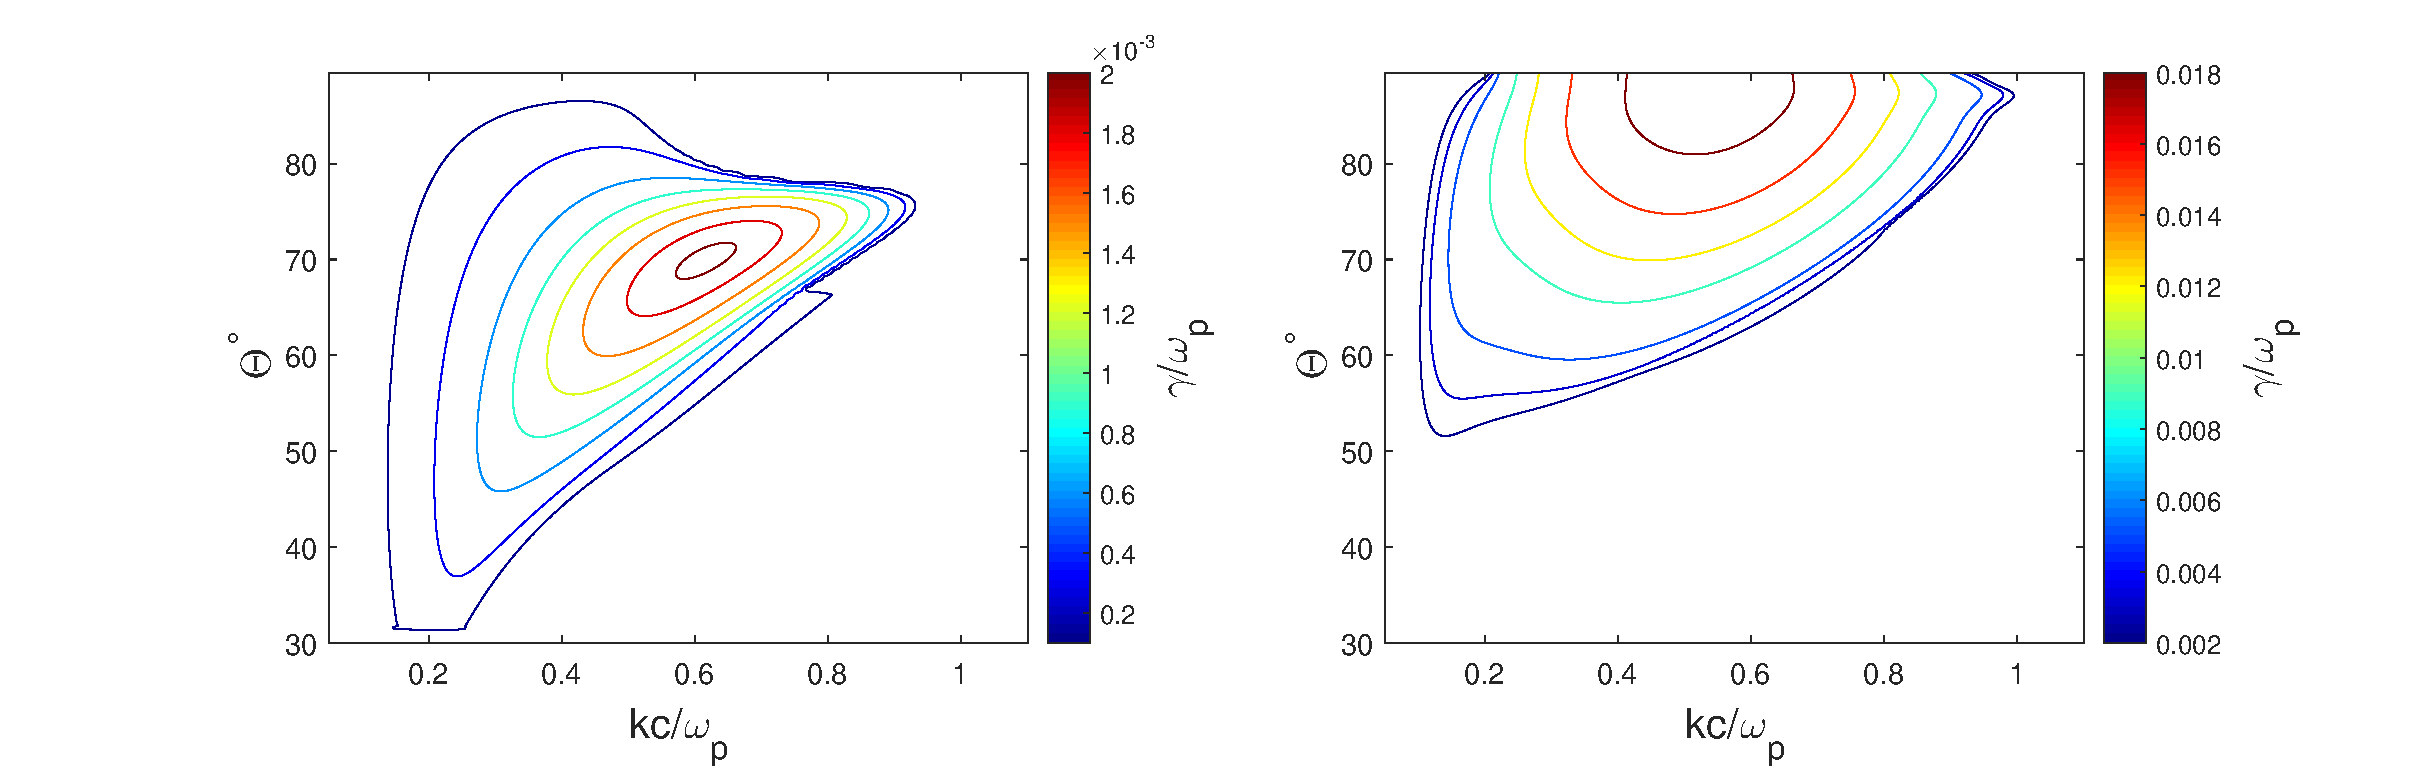
\includegraphics[width=1\linewidth]{part4/area_firehose_inst.eps}
\captionstyle{normal}
\caption{Линии уровня линейного инкремента вейбелевской (шланговой) неустойчивости для бимаксвелловского распределения электронов по скоростям с анизотропией $A_0=1$ при а) относительно слабом ($b_{ext}=0.14$) и б) сильном ($b_{ext}=0.63$) внешнем магнитном поле.}
\label{ris:area_firehose_inst}
\end{figure}

Область неустойчивости поперечных мод с увеличением внешнего поля достаточно быстро сужается,  как с длинноволновой, так и с коротковолновой стороны спектра, а линейный инкремент всех мод, остающихся неустойчивыми, уменьшается (рис. \ref{ris:spectr_inst}).
В работе~\cite{Emelyanov2023_Radiophys} в пределе $\gamma\ll K_\perp\beta_\perp$, реализующемся при невысокой начальной анизотропии ($A_0\lesssim1$), либо при высокой анизотропии и внешнем магнитном поле, близком к подавляющему, область неустойчивости поперечных мод оценивалась как:
\begin{equation}
    K_\perp\in\frac{2\sqrt{A_0}}{\sqrt{3}}\left(\cos\left[\frac{\pi+\arccos\left(\frac{b_{ext}}{b_{s\perp}(A_0)}\right)}3\right];\cos\left[\frac{\pi-\arccos\left(\frac{b_{ext}}{b_{s\perp}(A_0)}\right)}3\right]\right),
    \label{eq:border_perp_inst}
\end{equation}
где $b_{s\perp}(A_0)$~--- нормированное магнитное поле, подавляющее неустойчивость поперечных мод, квадрат которого оценен в~\cite{Emelyanov2023_Radiophys} как:
\begin{equation}
    b_{s\perp}^2(A_0)=\frac{8\pi}{27}\frac{A_0^3}{1+A_0^3}<1.
    \label{eq:Emel_condition}
\end{equation}
По мере увеличения внешнего магнитного поля $b_{ext}$ монотонно уменьшается не только линейный инкремент всех поперечных мод, но и угол между внешним магнитным полем и волновым вектором моды с наибольшим инкрементом~(рис. \ref{ris:spectr_inst})~\cite{Moya2022,Li2000,Camporeale2008}. 
Таким образом, для наклонных мод неустойчивость может развиваться при $b_{ext}>b_{s\perp}(A_0)$. 
Вводя величину магнитного поля $b_s(A_0)$, при которой апериодическая неустойчивость полностью подавлена, приведем оценку для неё из работы~\cite{Hellinger2014}, аппроксимирующую численно полученный порог неустойчивости в диапазоне значений начальной анизотропии $A_0$ от $0.2$ до $9$:

\begin{equation}
    b_{s}^2(A_0)=\left(\frac{A_0}{1.27(1+A_0)}\right)^{\frac1{0.954}}.
    \label{eq:Hellinger_condition}
\end{equation}
\begin{figure}[h]
\includegraphics[width=0.5\linewidth]{part4/b_podavl12.png}
\centering
\captionstyle{normal}
\caption{Зависимость подавляющего внешнего магнитного поля от начальной анизотропии для поперечных апериодических мод~(\ref{eq:Emel_condition}) (черный цвет), всех апериодических мод согласно оценке~(\ref{eq:Hellinger_condition}) (синий цвет) и согласно результатам расчетов~\cite{Moya2022} (красный цвет).}
\label{ris:B_podavl}
\end{figure}

Сравнение оценок (\ref{eq:Emel_condition}) и (\ref{eq:Hellinger_condition}) показывает, что если при высоких начальных анизотропиях отношение $b_{s}^2/ b_{s\perp}^2$ лишь немного превышает единицу, то при низких начальных анизотропиях оно может составлять несколько порядков~(рис. \ref{ris:B_podavl}). 
Значит, существует широкий диапазон параметров, в котором принципиально важен учет наклонных мод, так как поперечные моды устойчивы в линейном приближении.
 
Нелинейная эволюция турбулентности, развивающейся в отсутствие внешнего магнитного поля, исследована преимущественно с использованием численного метода частиц в ячейках~\cite{Kato2005,Borodachev2010,Ruyer2015,Lazar2022,Borodachev2016_Radiofiz,Romanov2004,Garasev2021}. 
Его недостатками являются высокий уровень шумов и необходимость использования больших вычислительных ресурсов. 
Альтернативный квазилинейный подход к исследованию этой турбулентности развит в главах \ref{ch:ch1} и \ref{ch:ch2} ограничен учетом только интегрального нелинейного взаимодействия всех мод (пространственных гармоник) посредством их влияния на усредненную по пространству компоненту функции распределения частиц по скоростям. 
В данном приближении комплексные частоты мод неявно задаются текущей формой этого распределения, т.е. динамика мод формально является линейной. 
На этом основании указанное взаимодействие между модами будем называть квазилинейным, а все остальные возможные взаимодействия~--- нелинейными.

Ранее было показано, что нелинейной эволюции подобной турбулентности в присутствии внешнего магнитного поля свойственно более медленное и не степенное увеличение характерного масштаба  с одновременным уменьшением угла $\theta_{opt}$ между наиболее энергонесущей модой и осью анизотропии~\cite{Camporeale2008,Hellinger2014}. 
В настоящей главе проведено детальное исследование влияния внешнего магнитного поля и начальной анизотропии распределения частиц в бесстолкновительной бимаксвелловской плазме на:
(a) величину  насыщающего неустойчивость среднеквадратичного магнитного поля,
(b) долговременную нелинейную эволюцию среднеквадратичного магнитного поля и его характерного масштаба, 
(с) законы роста/спадания его гармоник и нелинейное (резонансное) взаимодействие между ними, 
(d) форму усредненной по пространству самосогласованной функции распределения частиц по скоростям и параметр её анизотропии.

Ряд работ~\cite{Camporeale2008,Hellinger2014,Lopez2020,Lazar2023} посвящен изучению магнитной турбулентности, порождаемой электронной апериодической шланговой неустойчивостью. 
В них в силу выбранной геометрии описано развитие неустойчивых мод лишь в одном из двух перпендикулярных к внешнему полю и оси анизотропии направлений.
В таком случае без внешнего магнитного поля изотропизация распределения будет происходить не аксиально симметрично. 
Добавление внешнего магнитного поля, сонаправленного с осью анизотропии, неизбежно приводит к процессу, невозможному в полноценном трехмерном аксиально симметричном моделировании~--- ларморовскому вращению не аксиально симметричной функции распределения частиц (см. раздел \ref{ch:ch4/sec5}). 
Еще одним недостатком 2D3V-симуляций оказывается отсуствие трехволнового взаимодействия (см. раздел \ref{ch:ch4/sec7}).
Совокупность этих и ряда других причин приводит к значительным расхождениям в наблюдаемой динамике спектра в двумерных и трехмерных расчетах, в частности, в различной динамике характерных масштабов турбулентности уже на временах всего в $3-4$ раза более поздних, чем момент насыщения экспоненциального роста неустойчивости.

Следовательно, в данной главе анализ основан прежде всего на результатах трехмерного (3D3V) моделирования методом частиц в ячейках при помощи кода EPOCH~\cite{Arber2015}. 
Поскольку полноценные трехмерные расчеты требуют больших вычислительных затрат, целесообразно выяснить, какие параметры турбулентности и на каких временах могут быть определены из двумерных расчетов. 
С этой целью в работе проведено сравнение результатов расчетов в трехмерной (3D3V) и двух вариантах двумерной (2D3V) геометриях. 
Во всех случаях проводится динамический учет всех трех компонент скорости частиц $\vec{v}$ и зависящих от них полей.  
Ограничением в двумерных расчетах являются лишь исключенные зависимости исследуемых функций либо от координаты $y$  в $(x,z)$ -- геометрии, когда магнитное поле и ось анизотропии лежат в плоскости расчета $xz$, либо от координаты $z$ в аксиальной $z$-геометрии, когда магнитное поле и ось анизотропии ортогональны плоскости расчета $xy$.  

С учетом описанных ограничений, двумерные расчеты могут адекватно отражать качественную динамику спектра турбулентности, поэтому из-за трудоемкости полноценных трехмерных расчетов они остаются актуальными, проводились в настоящей главе и обсуждаются ниже вместе с результатами работ~\cite{Camporeale2008,Hellinger2014}, в которых также использовалось бимаксвелловское распределение частиц по скоростям в качестве начального.
В работе~\cite{Camporeale2008} подробно обсуждается симуляция с начальной анизотропией $A_0=1.85$ и внешним магнитным полем $b_{ext}\approx0.36\approx b_{s\perp}$, а в работе  \cite{Hellinger2014}~--- с начальной анизотропией $A_0=3.63$ и внешним магнитным полем $b_{ext}\approx0.7\lesssim b_{s}\approx0.77$.

В этой главе используются прежние обезразмеренные значения времени, волнового числа и амплитуд мод магнитного поля~(\ref{eq19plus1}).
Температура измеряется в энергетических единицах, т.е. с учетом постоянной Больцмана $k_B$. 
Для описания эволюции однородной компоненты распределения частиц по скоростям $f_0(t,\overrightarrow{\beta})=\iiint\limits^{\infty}_{-\infty}f(\vec{v},\vec{r}, t) d^3\vec{r}$ вводится относительная поправка к ней и эффективный параметр анизотропии:
\begin{equation}
\label{eq:relative_addition}
    \delta f_{0}(t,\overrightarrow{\beta})=\frac{f_0(t,\overrightarrow{\beta})-f_0(0,\overrightarrow{\beta})}{f_0(0,0)},\ A=\frac{2\iiint\limits^{\infty}_{-\infty}\beta_z^2f_{0}(\tau,\overrightarrow{\beta}) d\beta_x d\beta_yd\beta_z}{\iiint\limits^{\infty}_{-\infty}\left(\beta_x^2+\beta_y^2\right)f_{0}(\tau,\overrightarrow{\beta}) d\beta_x d\beta_y d\beta_z}-1 .   
\end{equation}
Кроме выявления динамики указанных величин~(\ref{eq:relative_addition}), представленные ниже расчеты призваны выявить закономерности в эволюции турбулентных магнитных и электрических полей и плотности тока электронов, а также пространственных спектров данной турбулентности.

Для изучения зависимости эволюции спектра магнитного поля и распределения частиц по скоростям от величины внешнего магнитного поля была проведена серия расчетов кодом EPOCH для начальной анизотропии, равной $A_0=10$ и $A_0=1$ при значениях внешнего магнитного поля, равных $b_{ext}=0$; $\approx 0.7b_{s\perp}$; $\approx b_{s\perp}$ и $\approx B_{s\perp}+0.5(b_s-b_{s\perp})$. 
Все качественные выводы о влиянии внешнего магнитного поля на турбулентность при различных начальных анизотропиях оказались идентичны, поэтому ниже обсуждаются преимущественно более показательные симуляции со сравнительно высокой начальной анизотропией $A_0=10$.
Количество квазичастиц в одной ячейке $N_p$, количество ячеек в трех ортогональных направлениях $N_{x,y,z}$ и длина одной ячейки $L_s$ в дебаевских радиусах указаны в таблице \ref{tab1} для всех $16$ симуляций, анализ которых приводится в работе.
\begin{table}
\begin{tabular}{ |p{1cm}||p{1cm}|p{1.5cm}|p{3cm}|p{1cm}|p{1cm}|   }
 \hline
 № & $A_0$ & $b_{ext}$ & $N_x\times N_y\times N_z$ & $L_s$ & $N_p$\\
 \hline
 $1$  & $10$ & $0$ & $150\times150\times200$ & $d_e$  & $800$ \\
 $2$  & $10$ & $0.4$ & $150\times150\times200$ & $d_e$  & $800$ \\
 $3$  & $10$ & $0.59$ & $150\times150\times200$ & $d_e$ & $800$ \\
 $4$  & $10$ & $0.71$ &  $150\times150\times200$ & $d_e$  & $800$ \\
 \hline
 $5$  & $10$ & $0$ &  $800\times1\times800$ & $d_e$  & $800$ \\
 $6$  & $10$ & $0.4$ & $600\times1\times600$ & $d_e$  & $800$ \\
 $7$  & $10$ & $0.59$ & $600\times1\times600$ & $d_e$  & $800$ \\
 $8$  & $10$ & $0.71$ & $600\times1\times600$ & $d_e$  & $800$ \\
 \hline
 $11$ & $1$ & $0$ & $150\times150\times150$ & $2.5d_e$  & $800$ \\
 $12$ & $1$ & $0.16$ & $150\times150\times150$ & $2.5d_e$  & $800$ \\
 $13$ & $1$ & $0.24$ & $150\times150\times150$ & $2.5d_e$  & $800$\\
 $14$ & $1$ & $0.43$ & $150\times150\times150$ & $2.5d_e$  & $800$ \\
 \hline
 $15$ & $1$ & $0$ & $400\times1\times400$ & $2d_e$  & $1600$ \\
 $16$ & $1$ & $0.16$ & $400\times1\times400$ & $2d_e$  & $1600$ \\
 $17$ & $1$ & $0.24$ & $400\times1\times400$ & $2d_e$  & $1600$ \\
 $18$ & $1$ & $0.43$ & $400\times1\times400$ & $2d_e$  & $1600$ \\
 \hline
 \end{tabular}
 \label{tab1}
 \caption{Таблица используемых в расчетах значений параметров}
\end{table}
Ниже при обсуждении результатов расчетов немаловажным является то обстоятельство, что с ростом внешнего магнитного поля монотонно уменьшается максимальный линейный инкремент апериодической неустойчивости, вследствие этого характерные времена развития турбулентности вырастают. 
Это отличие в значительной степени предопределяет разницу во временной динамике нижеобсуждаемых расчетов, проведенных при различных значениях внешнего магнитного поля. 

\section{Деформация распределения частиц в зависимости от величины  внешнего магнитного поля}
\label{ch:ch4/sec5}
В отсутствии внешнего магнитного поля и наклонных мод ранее наблюдалась значительная деформация функции распределения частиц на стадии насыщения экспоненциального роста во всей области скоростей порядка тепловых (глава \ref{ch:ch2}). 
В данном процессе происходит быстрое увеличение поперечной к оси анизотропии скорости электронов, двигавшихся сначала преимущественно вдоль этой оси, так что его форма принимает вид, существенно отличный от бимаксвелловского~(рис. \ref{ris:FR_A10_3d_B0}). 
В дальнейшем форма функции распределения частиц, остающаяся сильно не бимаксвелловской, изменяется медленно, квазилинейно, т.е. исключительно за счет интегрального нелинейного влияния мод на однородную компоненту функции распределения в условиях формально линейной эволюции каждой моды согласно текущему значению инкремента (декремента) и частоты (в общем случае ненулевой), определяемыми этой медленно меняющейся функцией распределения частиц. 
Это было показано сравнением симуляций методом частиц в ячейках с расчетами, учитывающими исключительно квазилинейное взаимодействие. 
На временах, по меньшей мере пятикратно превышающих момент окончания экспоненциального роста, учет наклонных мод и нелинейных взаимодействий, с ними связанных, в отсутствие внешнего магнитного поля не оказывает существенного влияния на эволюцию распределения частиц по скоростям за исключением, возможно, кратковременного переходного промежутка примерно от $\omega_pt=80$ до $\omega_pt=100$ при насыщении неустойчивости. 

\begin{figure}[h!]
\includegraphics[width=1\linewidth]{part4/FR_B0_A10_3d.png}
\captionstyle{normal}
\caption{Вычисленные для моментов времени (a)~$\wpl t = 88$, (b)~$\wpl t = 125.7$, (c)~$\wpl t = 854.5$ линии уровня $-0.5$, $-0.4$, $-0.3$, $-0.2$, $-0.1$, $0$, $0.05$ и $0.1$ нормированной на максимум начального распределения поправки к однородной компоненте функции распределения (\ref{eq:relative_addition}), которая в начальный момент времени являлась бимаксвелловской (\ref{eq:bimax}) с параметром анизотропии $A_0=10$. Внешнее магнитное поле отсутствует: $b_{ext}=0$.}
\label{ris:FR_A10_3d_B0}
\end{figure}

В присутствии внешнего магнитного поля $b_{ext}$, по-прежнему, непосредственно после насыщения линейной неустойчивости происходит сравнительно быстрое увеличение поперечной к оси анизотропии скорости части электронов, двигавшихся сначала преимущественно вдоль этой оси. 
По мере увеличения внешнего магнитного поля $B_{ext}$ количество таких электронов уменьшается. 
При его умеренном значении $b_{ext}=0.4$ область наибольшего приращения функции распределения электронов $\delta f_{0}(t,\overrightarrow{\beta})$ (\ref{eq:analit_estimation}) значительно деформируется, вытягиваясь вдоль ось анизотропии (рис.~\ref{ris:FR_A10_3d_B44}a). 
В сильном поле $b_{ext}=0.71$ в момент насыщения неустойчивости вышеобозначенная область значительно сдвигается, так что её характерная продольная скорость в момент насыщения неустойчивости вместо нуля равна $\beta_\|\sim3\beta_{\perp0}$, в то время как характерная поперечная скорость остается приблизительно равной $\beta_\perp\lesssim2\beta_{\perp0}$ (рис.~\ref{ris:FR_A10_3d_B78}a). 
Наиболее значительное уменьшение количества и в незамагниченной плазме, и в случае умеренного внешнего магнитного поля $b_{ext}=0.4$ наблюдается для электронов, исходно преимущественно сонаправленных с осью анизотропии, а именно обладающих продольной скоростью примерно от $\sim2\beta_{\perp0}$ до $\sim3\beta_{\perp0}$.
В случае поля $b_{ext}=0.71$ область оттока электронов значительно уже и занимает промежуток продольных скоростей от $\sim3\beta_{\perp0}$ до $\sim4\beta_{\perp0}$.

\begin{figure}[h!]
\includegraphics[width=1\linewidth]{part4/FR_B044_A10_3d.png}
\captionstyle{normal}
\caption{Вычисленные для моментов времени (a)~$\wpl t = 125.7$, (b)~$\wpl t = 314.2$, (c)~$\wpl t = 854.5$ линии уровня $-0.4$, $-0.3$, $-0.2$, $-0.1$, $0$, $0.025$ и $0.05$ нормированной на максимум начального распределения поправки к однородной компоненте функции распределения  (\ref{eq:relative_addition}), которая в начальный момент времени являлась бимаксвелловской (\ref{eq:bimax}) с параметром анизотропии $A_0=10$. Внешнее магнитное поле $b_{ext}=0.4$.}
\label{ris:FR_A10_3d_B44}
\end{figure}

В ходе дальнейшего нелинейного развития турбулентности в отсутствие внешнего магнитного поля форма ФР частиц по скоростям меняется слабо, преимущественно за счет нагрева в поперечном к оси анизотропии направлении электронов с малой продольной скоростью, что расширяет область значительного оттока частиц в диапазон малых скоростей $\left(\beta_\perp<\beta_{\perp0},\beta_\|<\beta_{\|0}\right)$ (рис. \ref{ris:FR_A10_3d_B0}c).
В умеренном внешнем магнитном поле $b_{ext}=0.4$ нелинейная динамика качественна схожа, но вышеописанный процесс ярче выражены количественно. 
В сильном внешнем магнитном поле $b_{ext}=0.71$ область значительного оттока частиц, абсолютный максимум которого достигается при $\beta_\|\sim3\beta_{\perp0}$, расширяется еще существеннее, так что появляется локальный максимум в области малых скоростей $\left(\beta_\perp<\beta_{\perp0},\beta_\|<\beta_{\|0}\right)$. 
А область наибольшего приращения функции распределения электронов $\delta f_{0}(t,\overrightarrow{\beta})$ расширяется вдоль оси анизотропии приблизительно от $\beta_\|\sim3\beta_{\perp0}$ до $\beta_\|\sim\beta_{\perp0}$. 
Из последующих разделов видно, что более значительная деформация распределения электронов в ходе долговременной нелинейной эволюции сильно замагниченной турбулентности взаимосвязана с более существенным изменением её спектральных характеристик. 

\begin{figure}[h!]
\includegraphics[width=1\linewidth]{part4/FR_B078_A10_3d.png}
\captionstyle{normal}
\caption{Вычисленные для моментов времени (a)~$\wpl t = 477.5$, (b)~$\wpl t = 628.3$, (c)~$\wpl t = 854.5$ линии уровня $-0.25$, $-0.2$, $-0.15$, $-0.1$, $-0.05$, $0$, $0.02$ и $0.04$ нормированной на максимум начального распределения поправки к однородной компоненте функции распределения (\ref{eq:bimax}), которая в начальный момент времени являлась бимаксвелловской с параметром анизотропии $A_0=10$. Внешнее магнитное поле $b_{ext}=0.71$.}
\label{ris:FR_A10_3d_B78}
\end{figure}

В двумерных расчетах 2D3V с магнитным полем, лежащим в плоскости моделирования, (как и в работах \cite{Camporeale2008,Hellinger2014}) функции распределения частиц по скоростям в плоскости, демонстрируют качественно схожую динамику, но с одним нюансом: утрата аксиальной симметрии возбуждаемым спектром квазимагнитостатического поля приводит к потере на нелинейной стадии аксиальной симметрии функцией распределения в ортогональной к внешнему магнитному полю и оси анизотропии плоскости. 
В случае незамагниченной плазмы это приводит к изотропизации исключительно в плоскости, определяемой волновым вектором и осью анизотропии.
В присутствии внешнего магнитного поля, сонаправленного с осью анизотропии, распределение частиц испытывает ларморовское вращение, вследствие чего развивающиеся исключительно в двумерной расчетной плоскости неустойчивые моды последовательно изотропизуют распределение частиц по скоростям во всех направлениях, ортогональных к оси анизотропии. 
В полноценном трехмерном расчете при равномерных начальных условиях симметрия нарастающего спектра по аксиальному углу сохраняется, так что обеспечивается аксиально симметричная изотропизация распределения частиц по скоростям, а значит, процесс, подобный описанному выше, исключен. 
Вследствие описанного выше различия, деформированные распределения электронов по скоростям (ср. рис. \ref{ris:FR_A10_2d_B78} и рис. \ref{ris:FR_A10_3d_B78}) и характеристики согласованного с ним спектра турбулентности (см. раздел \ref{ch:ch4/sec6}) могут существенно количественно различаться в двумерном и трехмерном расчетах, а значит, результаты подобного 2D3V моделирования лишь ограниченно применимы для анализа полноценной трехмерной задачи.

\begin{figure}[h!]
\includegraphics[width=1\linewidth]{part4/FR_2d B78_A10.png}
\captionstyle{normal}
\caption{Вычисленные с использованием 2D3V моделирования для моментов времени (a)~$\wpl t = 477.5$, (b)~$\wpl t = 628.3$, (c)~$\wpl t = 854.5$ линии уровня $-0.12$, $-0.08$, $-0.04$, $0$, $0.025$, $0.05$ нормированной на максимум начального распределения поправки к однородной компоненте функции распределения (\ref{eq:bimax}), которая в начальный момент времени являлась бимаксвелловской с параметром анизотропии $A_0=10$. Внешнее магнитное поле $b_{ext}=0.71$.}
\label{ris:FR_A10_2d_B78}
\end{figure}


Как и ранее в главах {\ref{ch:ch1} и \ref{ch:ch2}} с целью выявления доминирующего механизма на протяжении нелинейной эволюции квазимагнитостатической турбулентности было проведено сравнения результатов расчетов кодом EPOCH с результатами квазилинейного моделирования, в котором исключено прямое нелинейное взаимодействие между модами и оставлено лишь их взаимодействие посредством совместной деформации однородной в пространстве компоненты распределения частиц по скоростям.
Сравнение проведено в той же аксиально симметричной 2D3V геометрии, в которой были получены результаты в главе \ref{ch:ch2}, для умеренного значения внешнего магнитного поля $b_{ext}=0.4$.
В результате выявлено, что хотя к моменту насыщения неустойчивости указанные распределения частиц аналогичны, на более поздних временах они качественно отличаются в диапазоне малых скоростей  (ср. рис. \ref{ris:FR_A10_3d_B44_QL} и рис. \ref{ris:FR_A10_3d_B44}). 
Эта разница определяется существенно отличной динамикой спектра в обсуждаемых симуляциях (см. раздел \ref{ch:ch4/sec10}). 
Из этих различий следует, что квазилинейное приближение недостаточно для описания эволюции турбулентности  уже при довольно слабом внешнем магнитном поле, например, $b_{ext}=0.4$ при $A_0=10$. 
\begin{figure}[h!]
\includegraphics[width=0.7\linewidth]{part4/FR_QL_B4_A10.png}
\captionstyle{normal}
\centering
\caption{Вычисленные в квазилинейном аксиально симметричном приближении для моментов времени (a)~$\wpl t = 84$, (b)~$\wpl t = 92$, (c)~$\wpl t = 100$, (d)~$\wpl t = 420$ линии уровня $-0.5$, $-0.4$, $-0.3$, $-0.2$, $-0.1$, $0$, $0.05$ и $0.1$ нормированной на максимум начального распределения поправки к однородной компоненте функции распределения (\ref{eq:bimax}), которая в начальный момент времени являлась бимаксвелловской с параметром анизотропии $A_0=10$. Внешнее магнитное поле $b_{ext}=0.4$.}
\label{ris:FR_A10_3d_B44_QL}
\end{figure}

\section{Эволюция интегральных характеристик турбулентности при различных значениях внешнего магнитного поля}
\label{ch:ch4/sec6}

Параметр анизотропии $A$, будучи интегральным отражением формы распределения частиц, в отсутствие внешнего магнитного поля испытывает наиболее значительное снижение к моменту насыщения неустойчивости, а в сильном магнитном поле, равном, например, $b_{ext}=0.71$, ситуация противоположная и изотропизация распределения происходит преимущественно в ходе нелинейной эволюции (рис. \ref{ris:average_A10}c). 
Так, в первом случае к насыщению неустойчивости в $\tau_s=88$ анизотропия резко, примерно в 5 раз, уменьшается до $\approx2$, далее её снижение плавно замедляется и на временах $2\tau_s=176$ она составляет $A\approx1.1$. 
Во втором случае к моменту насыщения неустойчивости $\tau_s=390$ анизотропия снижается всего до $\approx7.2$, а на временах $2\tau_s=780$ составляет уже $A\approx3.83$.

Обращает на себя внимание то, что величина среднеквадратичного магнитного поля к концу симуляции в этих противоположных случаях различалась всего на $5 \%$ (рис. \ref{ris:average_A10}a,b). 
В отсутствие внешнего поля эта величина сравнительно быстро выросла, достигла насыщения и стала сравнительно быстро затухать. 
В сильном же внешнем поле апериодическая неустойчивость достигла своего насыщения в $4$ раза позднее и при в $3.5$ раза меньшем турбулентном магнитном поле, однако после этого  среднеквадратичное магнитное поле до конца симуляции находилось на примерно одном и том же уровне, что предопределило близость обсуждаемых величин к концу обеих симуляций. 
Полученное совпадение не выглядит случайным, так как среднеквадратичное магнитное поле в двух других расчетах с промежуточными значениями магнитного поля $b_{ext}=0.4$ и $b_{ext}=0.59$ к концу симуляции пришло к сравнимым значениям, отличающимся всего на $10 \%$ и $20 \%$ соответственно. 
Идентичный результат наблюдается и для аналогичных симуляций при начальной анизотропии $A_0=1$. 

\begin{figure}[h]
\includegraphics[width=1\linewidth]{part4/average_A10.jpg}
\captionstyle{normal}
\caption{Эволюция (a) поперечной и (b) продольной компонент среднеквадратичного магнитного поля $b_{av}$, (c) параметра анизотропии $A$, (d) поперечной компоненты храктерного волнового числа $\langle K_\perp\rangle$, а также характерной (e) поперечной $\langle \Delta K_\perp\rangle$ и (f) продольной $\langle \Delta K_\|\rangle$ ширины спектра при значениях внешнего магнитного поля $b_{ext}=0$ (синий цвет), $b_{ext}=0.4$ (красный цвет), $b_{ext}=0.59$ (зеленый цвет) и $b_{ext}=0.71$ (черный цвет) в трехмерных (сплошная линия), двумерных с наклонными модами (пунктир) и двумерных аксиально симметричных (штрихи) симуляциях. Начальная анизотропия равна $A_0=10$.}
\label{ris:average_A10}
\end{figure}

Во всех трехмерных симуляциях преобладает поперечная к оси анизотропии компонента магнитного поля, кратно, но не на порядки превосходя продольную компоненту. 
На протяжении нелинейной эволюции турбулентности их отношение уменьшается. 
Так, в отсутствие внешнего магнитного поля при насыщении неустойчивости их отношение примерно равно $b_\perp/b_\|\approx4$, на момент окончания расчета~--- $b_\perp/b_\|\approx3$, а в сильном внешнем магнитном поле $b_{ext}=0.71$ при насыщении неустойчивости их отношение примерно равно $b_\perp/b_\|\approx10$,  на момент окончания расчета~--- $b_\perp/b_\|\approx5$. 

Значение перпендикулярной компоненты характерного волнового числа $\langle K_\perp\rangle$ к моменту насыщения неустойчивости соответствуют волновому вектору наиболее неустойчивой моды, а значит, определяются линейной теорией. 
Здесь усреднение понимается в следующем смысле:
\begin{equation}
\label{eq:angles_b0}
\langle...\rangle=\frac{\iint\limits_0^\infty\int\limits_{-\infty}^\infty...b_K^2 dK_\|K_\perp dK_\perp}{\iint\limits_0^\infty\int\limits_{-\infty}^\infty b_K^2 dK_\|K_\perp dK_\perp}, 
\end{equation}
Волновое число наиболее неустойчивой моды $K_{opt}$ увеличивается c ростом внешнего магнитного поля, пока наиболее неустойчивыми модами остаются поперечные моды. 
При более высоких внешних магнитных полях $b_{ext}$ определяющими всю динамику турбулентности становятся наклонные моды, а поперечная компонента наиболее неустойчивой моды $K_{opt,\perp}$ снижается. 
В ходе последующей нелинейной эволюции поперечный масштаб турбулентности в каждом из случаев практически монотонно возрастает (рис. \ref{ris:average_A10}d), в то время как поперечная ширина спектра $\langle \Delta K_\perp\rangle$, где $\Delta K=K_\perp-\langle K_\perp\rangle$ остается примерно постоянной, равной примерно $\approx0.1$ в отсутствие внешнего магнитного поля, $\approx0.2$ при его умеренном значении $b_ext=0.4$, $\approx0.3$ при $b_ext=0.59,0.71$ (рис\ref{ris:average_A10}e).
Вследствие влияния внешнего магнитного поля на линейное дисперсионное соотношениe продольная ширина спектра $\langle \Delta K_\|\rangle=\langle  K_\|\rangle$ к моменту насыщения неустойчивости выше при более сильных магнитных полях.
При нелинейной эволюции эта величина возрастает вследствие нелинейного возбуждения разнообразных наклонных мод, устойчивых согласно линейной теории.
К концу симуляции во всех случаях продольный и поперечный масштабы оказывались сопоставимы, так что становится невозможно говорить о филаментационной структуре токов. 
В целом, результаты согласуются с~\cite{Hellinger2014,Camporeale2008}, отмечавшими увеличение масштаба турбулентности и уменьшение угла между внешним магнитным полем и характерным волновым вектором. 
Несмотря на хорошее количественное совпадение для всех четырех значений внешнего магнитного поля результатов эволюции параметра анизотропии (точность до 15\%) и среднеквадратичного магнитного поля (без случая $b_{ext}=0$ точность до 20 \%) у двумерных и трехмерных расчетов, сравнение в этих расчетах продольного и поперечного характерных масштабов турбулентности показывает, что на нелинейной стадии они значительно расходятся и могут кратно отличаться.  
Это существенно затрудняет изучение долговременной спектральной эволюции трехмерной турбулентности на основе анализа двумерных симуляций, как это, по-видимому, делается в указанных выше работах. 
Анализ спектральной динамики турбулентности, генерируемой шланговой модой, ниже основан на трехмерных симуляциях и посвящен преимущественно спектральной динамике поперечной компоненты магнитного поля, усредненной по аксильному углу. 
Усреднение приводит к сглаживанию шумов и осцилляций, наблюдаемых на стадии затухания мод, что позволяет оценить показатель степенного спадания их амплитуды.

\section{Динамика спектра вейбелевской турбулентности и нелинейное взаимодействие мод в отсутствие внешнего магнитного поля}
\label{ch:ch4/sec7}

В отсутствие наклонных мод и внешнего магнитного поля общий сценарий эволюции спектра вейбелевской турбулентности, который по существу можно назвать квазилинейным, был подробно описан в аксиально симметричной двумерной геометрии (все моды лежат в плоскости, ортогональной к оси анизотропии) в главе \ref{ch:ch2}, а также в работе~\ref{Kuznetsov2023}. 
При бимаксвелловском начальном распределении частиц неустойчивой оказывается исключительно ТМ-мода, магнитное поле которой ортогонально к плоскости опредлеляемой осью анизотропии и волновым вектором~\ref{fig:TMmodes}. 
После насыщения неустойчивости спектр магнитного поля, управляемый преимущественно квазилинейным взаимодействием, смещается в длинноволновую область так, что характерное волновое число уменьшается степенным образом, а степень наклона длинноволнового и коротковолнового хвостов остается примерно постоянной, что говорит об автомодельности динамики спектра. 
Единственным наблюдаемым нелинейным эффектом является развитие ТМ-гармоник, нечетным образом кратных к оптимальной, преимущественно утроенной гармоники~(рис. \ref{ris:triple_nonlinear}), генерируемой четырехволновым взаимодействием~\cite{Garasev2021,Kuznetsov2023}. 
Таким образом, были выделены 4 стадии эволюции ТМ-мод: экспоненциальный рост согласно линейному дисперсионному уравнению, степенной рост мод, волновое число которых меньше характерного $\langle K_\perp\rangle$, осцилляционное затухание мод, волновое число которых больше характерного $\langle K_\perp\rangle$, и сверхбыстрый нелинейный рост вследствие четырехволнового взаимодействия~(рис. \ref{ris:all_modes}a).  
Показатель степенного роста оценивался примерно от $1$ до $2$, а показатель затухания, которое после усреднения по аксиальному углу оказывалось степенным, лежал в небольшом диапазоне значений от $-1.3$ до $-1$ для широкого диапазона значений начальных анизотропий. 

\begin{figure}[h]
\includegraphics[width=1\linewidth]{part4/garmoniki_final.png}
\captionstyle{normal}
\caption{Эволюция типичных усредненных по аксиальному углу мод: примерно оптимальной моды $\overrightarrow{K}_{opt}$ (черный цвет); линейно неустойчивой моды, испытывающей степенное нарастание (синий цвет);  линейно устойчивых, затухающих непосредственно после сверхбыстрой генерации мод (красный цвет); линейно устойчивых, примерно степенным образом нарастающих после окончания сверхбыстрой генерации мод (зеленый цвет), наиболее энергонесущей моды с $K_\perp=0$ (бирюзовый цвет) при внешнем магнитном поле (a) $b_{ext}=0$, (b) $b_{ext}=0.4$. (c) $b_{ext}=0.59$, (d) $b_{ext}=0.71$. Вертикальный пунктир соответствует первому локальному максимуму среднеквадратичного магнитного поля в каждом случае. Начальная анизотропия $A_0=10$.}
\label{ris:all_modes}
\end{figure}

Другим нелинейным эффектом, который наблюдается в трехмерной (3D3V) геометрии, является трехволновая генерация линейно устойчивых ТЕ-мод, т.е. мод, электрическое поле которых ортогонально к плоскости, определяемой волновым вектором и осью анизотропиии, посредством взаимодействия двух апериодических неустойчивых ТМ-мод~(см. рис. \ref{ris:te_mode}). 
Этот эффект проявляется на стадии линейной неустойчивости при экспоненциальном росте ТЕ-мод с инкрементом, меньшим или порядка удвоенного максимального (точной оценке препятствует высокий уровень шумов). 
Область наблюдаемой генерации волновых чисел ТЕ-мод сравнима с областью линейно неустойчивых ТМ-мод, а оптимальная ТЕ-мода немного смещена в длинноволновую область относительно оптимальной ТМ-моды ($\approx20-30\%$). 
В двумерной (2D3V) геометрии (как в работах~\cite{Camporeale2008,Hellinger2014}) с наклонными модами подобное взаимодействие геометрически невозможно, поэтому продольная компонента магнитного поля отсутствует. 
\begin{figure}[h]
\includegraphics[width=0.5\linewidth]{part4/te_gener.eps}
\captionstyle{normal}
\centering
\caption{Трехволновая генерация наклонных линейно устойчивых ТE-мод. 
Синиим кругом обозначено множество мод, находящихся на коротковолновой границе области линейной неустойчивости, зеленым кругом обозначено множество мод с наибольшим линейным инкрементом $\gamma_{max}$, обладающих волновым вектором $|K_{opt}|$. 
Стрелками показаны линейно неустойчивые моды $\overrightarrow{K}_1$ и $\overrightarrow{K}_2$ (черный цвет) и нелинейно генерируемая мода с волновым вектором, равным $\overrightarrow{K}_1-\overrightarrow{K}_2$ (красный цвет).
}
\label{ris:te_mode}
\end{figure}


Добавление наклонных мод еще сильнее увеличивает разнообразие и влияние нелинейных взаимодействий, из-за которых наблюдается нелинейный сверхбыстрый рост не только поперечных ТМ-мод коротковолнового крыла, но и широкого разнообразия наклонных ТМ-мод~(рис. \ref{ris:oblique_wave}), инкремент которых, согласно линейной теории для текущего распределения частиц, близок к нулю или вовсе отрицателен~(рис. \ref{ris:spectrA10_B0}). 
Хотя квазилинейное взаимодействие, по-видимому, продолжает играть важную роль, спектральная динамика существенно перестает быть квазилинейной: спектр турбулентности за счет прямых нелинейных взаимодействий между гармониками расширяется вдоль оси анизотропии, а среднеквадратичное магнитное поле затухает значительно быстрее, чем в аксиально симметричных расчетах без учета наклонных мод.
\begin{figure}[h]
\includegraphics[width=0.5\linewidth]{part4/oblique_mode_generation.eps}
\captionstyle{normal}
\centering
\caption{Трехволновая генерация наклонных линейно устойчивых ТМ-мод. Линии уровня инкрементов аналогичны рис.~\ref{ris:area_firehose_inst}a.
Стрелками показаны линейно неустойчивые моды $\overrightarrow{K}_1$ и $\overrightarrow{K}_2$ (черные сплошные), сопряженная с $\overrightarrow{K}_2$ линейно неустойчивая мода (черная сплошная) и нелинейно генерируемая мода с волновым вектором, равным $\overrightarrow{K}_1-\overrightarrow{K}_2$ (красный цвет).}
\label{ris:oblique_wave}
\end{figure}



\begin{figure}[h]
\includegraphics[width=0.5\linewidth]{part4/triple_mode_generation.eps}
\captionstyle{normal}
\centering
\caption{Четырехволновая генерация утроенных мод. Линии уровня инкрементов аналогичны рис.~\ref{ris:area_firehose_inst}a 
Стрелками показаны линейно неустойчивые моды $\overrightarrow{K}_1$ (черный цвет) и нелинейно генерируемая мода с волновым вектором, равным $3\overrightarrow{K}_1$ (красный цвет).}
\label{ris:triple_nonlinear}
\end{figure}

\begin{figure}[h]
\includegraphics[width=1\linewidth]{part4/srez_spectrA10_B0.eps}
\captionstyle{normal}
\caption{Распределение десятичных логарифмов амплитуд пространственных мод, $|b_K|$, усредненных по аксиальному углу, согласно расчетам на временах (a) $\omega_p\tau=88$, (b) $\omega_p\tau=125.7$, (c) $\omega_p\tau=854.5$ при внешнем магнитном поле $b_{ext}=0.4$.}
\label{ris:spectrA10_B0}
\end{figure}


Как и в двумерной аксиально симмтеричной задаче, рассмотренной в главе~\ref{ch:ch2}, гармоники могут находиться на одной из 4 возможных стадий эволюции: экспоненциальный, степенной или сверхбысрый рост, а также осцилляционное затухание. 
Показатель степенного роста, который могут испытывать и нелинейно индуцированные сравнительно длинноволновые наклонные гармоники, по-прежнему оценивается от $1$ до $2$. 
Усреднение по аксиальному углу позволяет также выделить показатель усредненного затухания, который после добавления наклонных мод увеличивается примерно в $1.5$ раз и теперь оценивается от $-2$ до $-1.5$.  

В незамагниченной плазме продольная компонента турбулентного магнитного поля возникает исключительно вследствие нелинейной генерации. 
Во внешнем магнитном поле неустойчивая апериодическая мода обладает смешанной поляризацией (ни ТМ- ни ТЕ-), что существенно сближает и без того схожую и взаимосвязанную спектральную динамику поперечной и продольной компонент магнитного поля. 
Поэтому в последующих главах обсуждается спектр именно поперечной компоненты турбулентного магнитного поля. 

\section{Конкуренция вейбелевской и шланговой турбулентности и нелинейное взаимодействие мод в сравнительно слабом внешнем магнитном поле}
\label{ch:ch4/sec8}
Уже при $b_{ext}< b_{s\perp}$ значение линейного инкремента может оказаться существенно выше у наклонных мод апериодической неустойчивости, чем у поперечных мод, а значит, неучет наклонных мод становится невозможен. 
При сравнительно слабом внешнем магнитного поля $b_{ext}=0.4$~(рис. \ref{ris:spectrA10_B44}) инкремент поперечных мод все еще сравним с максимальным, но область неустойчивости как в поперечном, так и в продольном к оси анизотропии направлениях существенно уменьшается~\cite{Emelyanov2023_Radiophys,Moya2022}, а длинноволновая граница области неустойчивости становится отличной от нуля~(\ref{eq:border_perp_inst}).
Помимо этого, апериодические неустойчивые моды теперь являются смешанными, то есть не являются ни ТЕ-, ни ТМ-модами. 

\begin{figure}[h]
\includegraphics[width=1\linewidth]{part4/srez_spectrA10_B44.eps}
\captionstyle{normal}
\caption{Распределение десятичных логарифмов амплитуд пространственных мод, $|b_K|$, усредненных по аксиальному углу, согласно расчетам на временах (a) $\omega_p\tau=125.7$, (b) $\omega_p\tau=314.2$, (c) $\omega_p\tau=854.5$ при внешнем магнитном поле $b_{ext}=0.4$.}
\label{ris:spectrA10_B44}
\end{figure}


Из-за нелинейной генерации мод в длинноволновом диапазоне~(рис. \ref{ris:oblique_wave}), спектр турбулентности вскоре после насыщения неустойчивости сравнительно быстро расширяется в эту область~(рис. \ref{ris:spectrA10_B44}). 
Подобная сверхбыстрая генерация длинноволновых, линейно устойчивых мод, которые уже на временах, двукратно превосходящих время насыщения неустойчивости, становятся основными энергонесущими модами, отсутствует в квазилинейном приближении, что предопределяет отличную эволюцию спектра. 
В квазилинейных аксиально симметричных симуляциях наблюдаются лишь не затухающие колебания линейно неустойчивых мод, а смещение спектра за пределы области линейной неустойчивости отсутствует (ср. рис. \ref{fig:anom_spectr}d и рис. \ref{fig:anom_spectr}f). 
Поэтому на временах уже двукратно превышающих момент насыщения неустойчивости спектр существенно не квазилинеен, что отражается на распределении частиц по скоростям~(ср. рис. \ref{ris:FR_A10_3d_B44} и рис. \ref{ris:FR_A10_3d_B44_QL}).

Тем не менее, многие черты квазилинейной эволюции спектральная динамика сохраняет: характерное волновое число по-прежнему смещается в длинноволновую область;  более коротковолновые моды, чем характерная в данный момент времени мода, осцилляционно затухают, а многие более длинноволновые, в том числе и нелинейно индуцированные при насыщении неустойчивости~--- нарастают по степенному закону. 
Затухание линейно неустойчивых гармоник замедляется в сравнении со случаем отсутствия внешнего магнитного поля и показатель их усредненного степенного затухания оценивается от $-1.3$ до $-0.8$. 
Показатели степенного нарастания основных энергонесущих гармоник по-прежнему лежат в промежутке от $1$ до $2$, в том числе и для некоторых нелинейно индуцированных длинноволновых мод. 
Исключением из обеих оценок являются длинноволновые, почти поперечные, нелинейно индуцированные моды $\left(K_x\lesssim0.6,K_y\lesssim0.1\right)$, показатели нарастания и затухания которых стремятся к нулю. 
Таким образом, хотя квазилинейное взаимодействие по-прежнему остается весьма существенным в присутствии внешнего магнитного поля, непосредственно вид наблюдаемого спектра турбулентного магнитного поля в значительной степени определяется прямым межмодовым нелинейным взаимодействием (рис.~\ref{ris:oblique_wave} и \ref{ris:te_mode}).

\section{Динамика спектра шланговой турбулентности и нелинейное взаимодействие мод в подавляющем поперечные моды внешнем магнитном поле}
\label{ch:ch4/sec9}

Начиная с величины внешнего магнитного поля $b_{ext}=0.59$ анализ линейного дисперсионного соотношения предсказывает устойчивость поперечных мод~(рис. \ref{ris:spectrA10_B65}). 
Оптимальный волновой вектор (волновой вектор с наибольшим линейным инкрементом) при $b_{ext}=0.59$ образует угол с осью анизотропии, приблизительно равный $77^\circ$, а область апериодической неустойчивости продолжает обужение как в продольном, так и в поперечном направлении. 
Топология области неустойчивости в трехмерном пространстве изменилась: ранее она состояла из одной связанной области, ограниченной квазитороидальной поверхностью, а теперь~--- из двух~(рис. \ref{ris:area_firehose_inst}). 
В ходе нелинейной динамики спектра, как и в работах~\cite{Camporeale2008,Hellinger2014}, наблюдается смещение его максимума в длинноволновую область и уменьшение отношения характерного поперечного волнового числа к продольному. 

\begin{figure}[h]
\includegraphics[width=1\linewidth]{part4/srez_spectrA10_B65.eps}
\captionstyle{normal}
\caption{Распределение десятичных логарифмов амплитуд пространственных мод, $|b_K|$, усредненных по аксиальному углу, согласно расчетам на временах (a) $\omega_p\tau=226.2$, (b) $\omega_p\tau=314.2$, (c) $\omega_p\tau=854.5$ при внешнем магнитном поле $b_{ext}=0.59$.}
\label{ris:spectrA10_B65}
\end{figure}

На протяжении нелинейной эволюции существенны квазипоперечные моды  $\left(K_\|<K_{\|opt}/2\right)$, генерируемые в широком диапазоне волновых чисел за счет трехволнового взаимодействия линейно неустойчивых мод~(\ref{ris:zero_generation}) и нарастающие с инкрементами, близкими к удвоенному максимальному инкременту~(рис. \ref{ris:all_modes}c).
В двухмерных расчетах, очевидно, учитывающих наклонные моды, подобный процесс приводит лишь к сравнительно слабой генерации поперечных мод с волновым числом приблизительно равным $K_\perp\approx2K_{\perp opt}$. 
В то же время в полноценных $3D3V$ симуляциях, помимо трехволнового взаимодействия в удобных для изображения плоскостях $Oxz$ на рис.~\ref{ris:zero_generation} и $Oxy$ на рис.~\ref{ris:te_mode}, оказывается возможным трехволновое взаимодействие в любой промежуточной плоскости, что подтверждается генерацией квазипоперечных мод с примерно удвоенными нелинейными инкрементами почти при любых значениях волновых чисел в промежутке от $0$ до $2K_\perp opt$~(рис. \ref{ris:spectrA10_B65}).
К моменту насыщения неустойчивости амплитуда их магнитного поля в $2-4$ раза ниже амплитуды магнитного поля наиболее линейно неустойчивой моды, а на временах в $3-4$ раза более поздних они становятся основными энергонесущими модами. 
Моды с удвоенной к линейно неустойчивым модам продольной компонентой волнового вектора $\left(K_\|\approx2K_{\|opt}\right)$ генерируются за счет того же механизма в широком, сравнимом с областью линейной неустойчивости, диапазоне значений поперечной компоненты~(рис. \ref{ris:area_firehose_inst}). 
Аналогично, к моменту насыщения неустойчивости их амплитуда в $2-4$ раза ниже амплитуды наиболее линейно неустойчивых мод. 
В течение последующей эволюции часть из них может стать основными энергонесущими модами, но к концу симуляций наблюдается затухание удвоенных продольных мод. 

\begin{figure}[h]
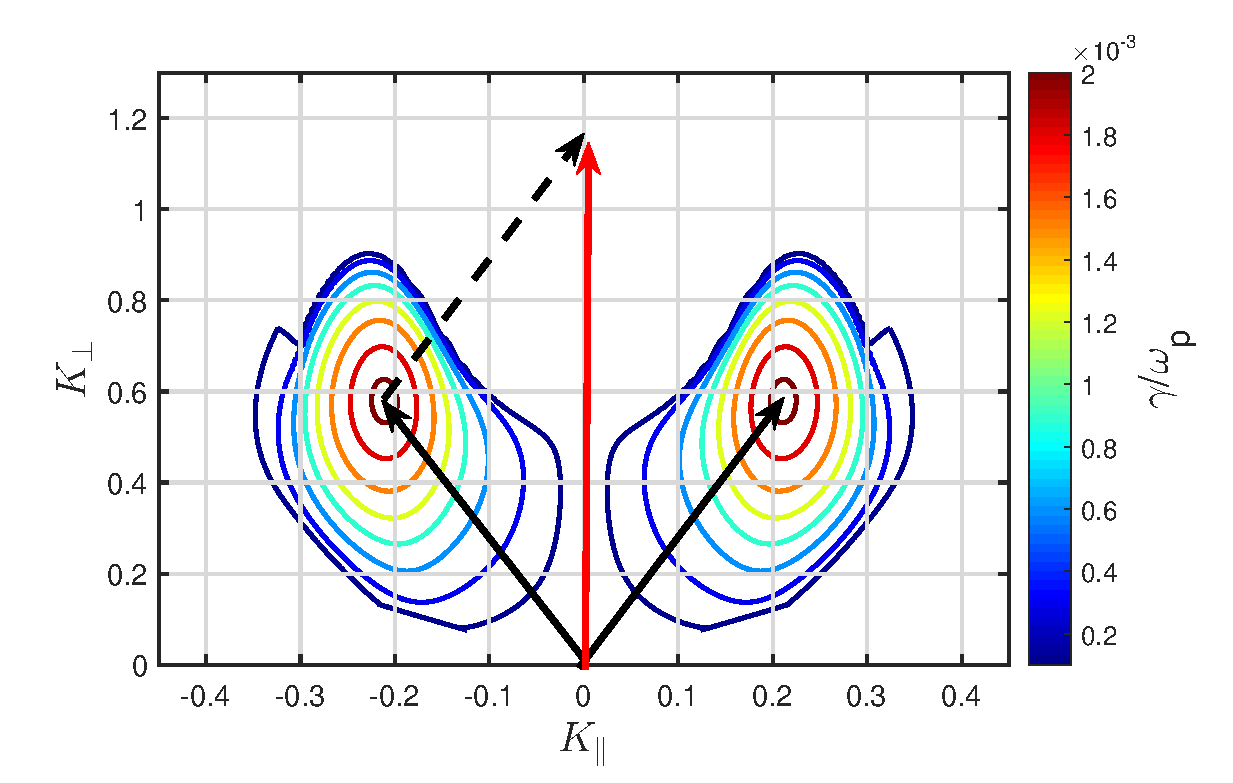
\includegraphics[width=0.5\linewidth]{part4/zero_mode_generation_high_b.eps}
\captionstyle{normal}
\centering
\caption{Трехволновая генерация поперечных к оси анизотропии линейно устойчивых мод. 
Линии уровня инкрементов аналогичны рис.~\ref{ris:area_firehose_inst}b.
Стрелками показаны линейно неустойчивые моды $\overrightarrow{K}_1$ и $\overrightarrow{K}_2$ (черные сплошные) и нелинейно генерируемая мода с ортогональным к оси анизотропии волновым вектором, равным $\overrightarrow{K}_1-\overrightarrow{K}_2$ (красный цвет).}
\label{ris:zero_generation}
\end{figure}

\begin{figure}[h]
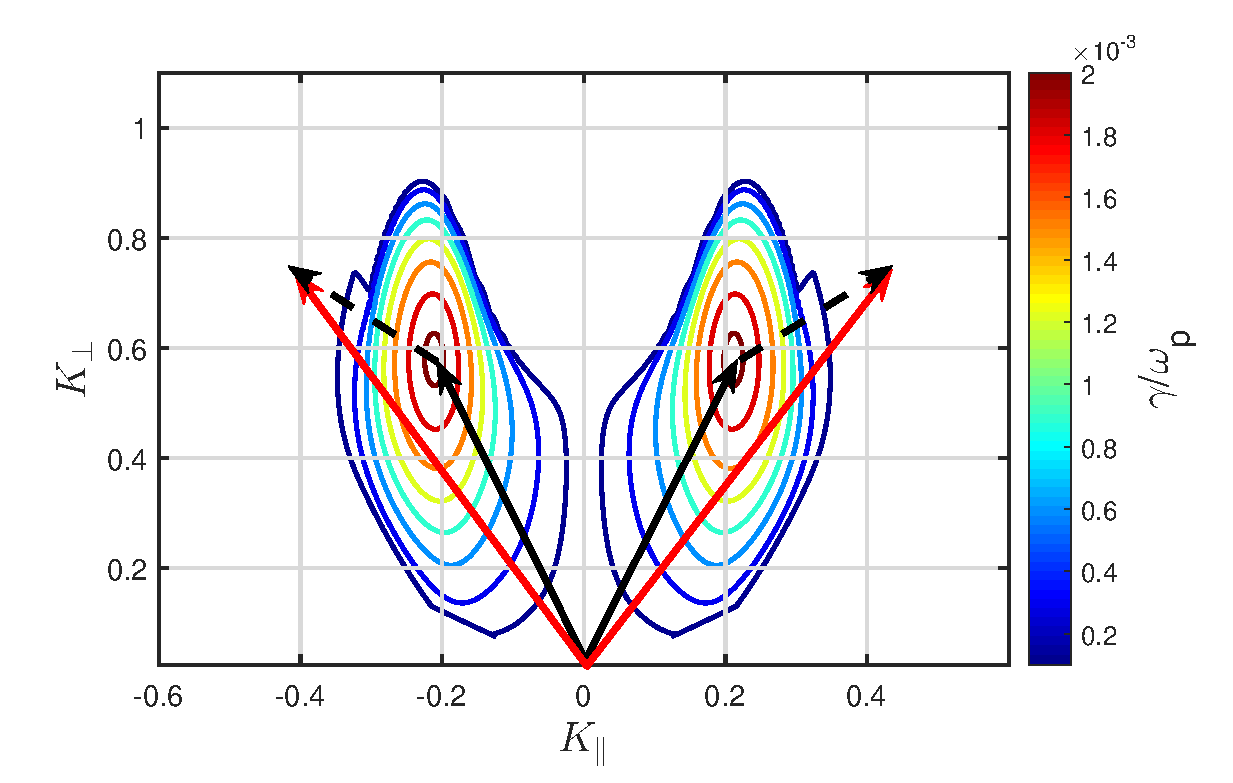
\includegraphics[width=0.5\linewidth]{part4/double_mode_generation_high_b.eps}
\captionstyle{normal}
\centering
\caption{Трехволновая генерация линейно устойчивых удвоеных мод. Линии уровня инкрементов аналогичны рис.~\ref{ris:area_firehose_inst}b.
Стрелками показаны линейно неустойчивые моды $\overrightarrow{K}_1$ и $\overrightarrow{K}_2$ (черные сплошные), сопряженная с $\overrightarrow{K}_2$ линейно неустойчивая мода (черная сплошная) и нелинейно генерируемая мода с волновым вектором, равным $\overrightarrow{K}_1-\overrightarrow{K}_2$ (красный цвет).
}
\label{ris:double_generation}
\end{figure}
По-прежнему выделяются 4 возможные стадии эволюции для гармоник. 
Линейно неустойчивые апериодические моды испытывают экспоненциальный рост в соответствии с дисперсионным соотношением. 
После насыщения своего роста каждая мода в отдельности осцилляционно затухает. 
При насыщении неустойчивости наблюдается сверхбыстрый рост поперечных и удвоенных продольных мод. 


В ходе дальнейшей нелинейной эволюции из-за деформации однородной компоненты функции распределения частиц по скоростям наблюдается примерно степенной рост сравнительно длинноволновых, изначально линейно устойчивых и не генерируемых нелинейно мод, с достаточно высокими показателями роста, близкими к 5. 
Область волновых чисел, в которой наблюдается степенной рост, можно грубо оценить: $K_{\|opt}\lesssim  K_\|\lesssim 2K_{\|opt}$, $0\lesssim K_\perp\lesssim 2K_{\perp opt}$. 
В работах~\cite{Camporeale2008,Hellinger2014} предполагается, что длинноволновое смещение спектра с уменьшением угла наклона между характерным волновым вектором и магнитным полем происходит квазилинейно, и предпринимаются попытки его объяснить на основе линейной теории. 
Важно, что скорость их степенного роста сравнима со скоростью экспоненциального роста линейно неустойчивых мод (а при внешнем поле $b_{ext}=0.71$ значительно превосходит), что кажется невероятным в контексте квазилинейного взаимодействия, так как наблюдаемое нарастание происходит при уже значительно изотропизованном распределении частиц по скоростям. 


\section{Шланговая турбулентность и нелинейное взаимодействие мод в сильном внешнем магнитном поле}
\label{part_spectr_b78}

Оптимальный волновой вектор линейного роста апериодической неустойчивости при  $b_{ext}=0.71$ образует угол с осью анизотропии, приблизительно равный  $70^\circ$, а область неустойчивости крайне обужена около соответствующей моды. 
К моменту насыщения неустойчивости наблюдается нелинейная генерация не только поперечных и удвоенных продольных мод, но и гармоник с примерно утроенным и даже учетверенным оптимальным продольным волновым числом~(рис. \ref{ris:all_modes}d), что придает спектру вдоль оси анизотропии гребенчатую форму. 
Далее в ходе нелинейной эволюции поперечное волновое число наиболее энергонесущих мод уменьшается, а продольное~--- увеличивается. 
Вслед за спектральным смещением наиболее энергонесущих мод происходит пропорциональное смещение кратных индуцированных гармоник. Вследствие этого спектр сглаживается в продольном направлении, теряя гребенчатую форму. 
Подобный процесс происходил и при меньшем поле $b_{ext}=0.59$, но был менее заметен из-за скоротечности и более широкого спектра линейно неустойчивых мод.


\begin{figure}[h]
\includegraphics[width=1\linewidth]{part4/srez_spectrA10_B78.eps}
\captionstyle{normal}
\caption{Распределение десятичных логарифмов амплитуд пространственных мод, $|b_K|$, усредненных по аксиальному углу, согласно расчетам на временах (a) $\omega_p\tau=477.5$, (b) $\omega_p\tau=628.3$, (c) $\omega_p\tau=854.5$ при внешнем магнитном поле $b_{ext}=0.71$.}
\label{ris:spectrA10_B78}
\end{figure}

На протяжении линейной неустойчивости происходит экспоненциальный рост смешанных апериодических мод в соответствии с линейной теорией. 
При насыщении неустойчивости наблюдается нелинейная генерация квазипоперечных $\left(K_\|<K_{\|opt}/2\right)$, удвоенных $\left(K_\|\approx2K_{\|opt}\right)$ и утроенных $\left(K_\|\approx3K_{\|opt}\right)$ продольных гармоник, а также гармоник на коротковолновом хвосте области неустойчивости $\left(K_\|\approx K_{\|opt},K_\perp\gtrsim2K_{\perp opt}\right)$. 
Квазипоперечные моды нарастают с инкрементами, близкими к удвоенным вследствие трехволнового взаимодействия. 
Подобно четырехволновой генерации утроенной моды в отсутствие внешнего магнитного поля~(рис. \ref{ris:triple_nonlinear}), для нелинейной генерации гармоник на коротковолновом хвосте линейной области неустойчивости должны сложится три основные энергонесущие моды. 
Инкременты нелинейного роста удвоенных продольных мод оценить затруднительно из-за шумов, однако они оказывается существенно выше удвоенного линейного, что дает основание предполагать генерацию этих гармоник не только посредством простого сложения двух линейно неустойчивых мод, но и за счет нелинейных взаимодействий более высокого порядка. 
То же касается и генерации утроенной продольной моды (рис. \ref{ris:all_modes}d). 
К насыщению неустойчивости уровень квазипоперечных и удвоенных продольных мод примерно на порядок ниже основной энергонесущей моды, утроенной продольной~--- на два порядка, гармоник коротковолнового хвоста~--- примерно полтора порядка. 
В ходе нелинейного смещения максимума спектра в линейно устойчивую область происходит быстрая, нелинейная генерация мод, отдельные участки которой лучше аппроксимируются экспоненциальной функцией, а отдельные~--- степенной с показателем, достигающим $10$. 


По мере роста величины внешнего магнитного поля наблюдается увеличивается разнообразие и глубина нелинейных явлений. 
В его отсутствие нелинейные явления сводятся к слабо влияющим на форму спектра трехволновой генерации TE-моды, четырехволновой генерации коротковолновых мод и нелинейной генерации наклонных мод. 
Влияние первого процесса сводится к появлению сонаправленной с внешним магнитным полем компоненты турбулентного поля, на порядок уступающего по величине его поперечной компоненте.
Влияние второго процесса преимущественно сказывается лишь на коротковолновом крыле спектра (см. раздел \ref{sec:ch2/sec2}). 
Последний процесс представляется наиболее значимым и приводящим как в соответствующих двумерных расчетах, так и в трехмерных к значительному ускорению затухания среднеквадратичного турбулентного магнитного поля.
При добавлении умеренного магнитного поля, равного, например, $b_{ext}=0.4$ при начальной анизотропии $A_0=10$ влияние нелинейных взаимодействий значительно усиливается и приводит к смещению спектра в линейно устойчивую область волновых чисел.
При внешнем магнитном поле $b_{ext}=0.59$, подавляющем линейный рост поперечных вейбелевских мод, в дополнение к ранее описанным явлениям ярко выраженным нелинейным эффектом оказывается нелинейная генерация последних.
Наконец, при внешнем магнитном поле $b_{ext}=0.71$ вследствие вышеописанных нелинейных взаимодействий формируется гребенчатый спектр вдоль оси анизотропии.

\section{Квазилинейное моделирование вейбелевской/шланговой турбулентности за пределами квазилинейного приближения}
\label{ch:ch4/sec10}
Различные плазменные среды, в которых развилась квазимагнитостатическая турбулентность вейбелевского типа, будучи бесстолкновительными или слабо столкновительными, демонстрируют явления, напоминающие обычные столкновительные взаимодействия. 
Это происходит потому, что мелкомасштабные поля в вейбелевской турбулентности меняются на масштабах, меньших или сравнимых с характерным радиусом кривизны траектории частицы, движущейся в поле, то есть с ларморовским радиусом частицы. 
Следовательно, даже если средняя намагниченность существенна и частица в основном движется вдоль своей ларморовской орбиты, сильные флуктуации напряженности поля в определенных областях могут нарушать адиабатический инвариант частицы, что приводит к питч-угловому рассеянию~\cite{Fleishman2013,Medvedev2017,Keenan2013,Keenan2015,Emelyanov2025}. 

В работе \cite{Emelyanov2025} показано, что вышеописанные аномальные столкновения частиц, обусловленные рассеянием на мелкомасштабных флуктуациях развитой вейбелевской турбулентности, приводят к сверхэкспоненциальному нарастанию длинноволновых гармоник, устойчивых в линейном приближении.
Этот результат согласуется с наблюдаемой при умеренном магнитном поле $b_{ext}=0.4$, при котором поперечные моды остаются неустойчивыми, нелинейной генерацией длинноволновых мод (рис.\ref{ris:spectrA10_B44}).  
Как было показано в главе \ref{ch:ch1}, явный учет прямого нелинейного взаимодействия гармоник для каждой неоднородной моды в следующем порядке малости приводит к стремительному росту числа уравнений в квазилинейном подходе, поэтому представляется невозможным.
Следовательно, целесообразен ввод аномальных столкновений в уравнения для периодических мод функции распределения частиц по скоростям (\ref{eq:f1.4_anom}) в простейшем БГК $\tau$-приближении~\cite{Bhatnagar1954,Medvedev2017} с целью эффективного учета нелинейного рассеяния распределения частиц каждой моды на квазимагнитостатических полях оставшихся мод.
Описанный подход реализован в задаче о двумерной аксиально-симметричной вейбелевской турбулентности магнитоактивной плазмы на основе квазилинейной системы уравнений (\ref{eq:f0.4})-(\ref{eq:maxw3.3}) с оператором (\ref{eq:oper.4}).

\begin{align}
\label{eq:f0.4_anom}
\dfrac{\partial \psi_0}{\partial \tau}+\sum\limits^{m}_{n=1}\mathrm{Re}\Bigg[\hat \Theta_1\left(e_{\vec{K}_{\vec{n}}},{\vec{b}}_{\vec{K}_{\vec{n}}},\psi_{K_n}^*\right)\Bigg]+\mathrm{Re}\Bigg[\hat \Theta_1\left(0,{\vec{b}}_{ext},\psi_{0}\right)\Bigg]=0,\\
\label{eq:f1.4_anom}
\dfrac{\partial \psi_{\overrightarrow{K}_{\vec{n}}}}{\partial \tau}+\mathrm{i}\overrightarrow{K}_{\vec{n}}\overrightarrow{\beta}\psi_{K_n}+2\hat \Theta_1\left(e_{\vec{K}_{\vec{n}}},{\vec{b}}_{\vec{K}_{\vec{n}}},\psi_{0}\right)+2\hat \Theta_1\left(0,{\vec{b}}_{ext},\psi_{\overrightarrow{K}_{\vec{n}}}\right)+\nu\psi_{\overrightarrow{K}_{\vec{n}}}=0,\\
\label{eq:maxw3.3_anom}
\dfrac{\partial e_{\vec{K}_{\vec{n}}}}{\partial \tau}=\mathrm{i}\left({b}_{\vec{K}_{\vec{n}}}\right)_x\left(K_{\vec{n}}\right)_z-\mathrm{i}\left({b}_{\vec{K}_{\vec{n}}}\right)_z\left(K_{\vec{n}}\right)_x+\beta_{\|0}^{-1}{\iiint\limits^{+\infty}_{-\infty}\beta_y\psi_{\vec{K}_{\vec{n}}}(\tau,\overrightarrow{\beta})d^3\beta} ,\\
\label{eq:oper.4_anom}
\hat \Theta_1\left(e_{\vec{K}_{\vec{n}}},{\vec{b}}_{\vec{K}_{\vec{n}}},\psi(\beta)\right)  =  \dfrac{e_{\vec{K}_{\vec{n}}}}{2}\dfrac{\partial \psi(\beta)}{\partial \beta_y}-\dfrac{\left({b}_{\vec{K}_{\vec{n}}}\right)_z}{2} \left(\beta_x\dfrac{\partial \psi(\beta)}{\partial \beta_y}-\beta_y\dfrac{\partial \psi(\beta)}{\partial \beta_x}\right) \nonumber \\
-\dfrac{\left({b}_{\vec{K}_{\vec{n}}}\right)_x}{2} \left(\beta_z\dfrac{\partial \psi(\beta)}{\partial \beta_x}-\beta_x\dfrac{\partial \psi(\beta)}{\partial \beta_z}\right) .
\end{align}
В замкнутой системе уравнений (\ref{eq:f0.4_anom})-(\ref{eq:f1.4_anom}) с оператором (\ref{eq:oper.4_anom}), следуя работам \cite{Fleishman2013,Medvedev2017,Keenan2013,Emelyanov2025}, введена нормированная на плазменную частоту $\omega_p$ частота аномальных столкновений $\nu$ в виде:
\begin{equation}
\nu=\alpha\omega_B^2\frac{\lambda_{cor}}{v_{\|}}=\frac{3\pi}{8}\sqrt{\frac32}\frac{\beta_{\|0}^2\langle |K|\rangle b_{av}^2}{\langle K^2\rangle\beta_{\|}},
\label{eq:anom_collisions}
\end{equation}
где $\alpha$~--- числовой коэффициент, $\lambda_{cor}$~--- корреляционная длина магнитных возмущений, $\omega_B$~--- гирочастота в среднеквадратичном магнитном поле $b_av$. 

Как и ранее численные решения представленной системы уравнений (\ref{eq:f0.4_anom})-(\ref{eq:f1.4_anom}) с оператором (\ref{eq:oper.4_anom}) были получены путем стандартного метода Стёрмера~-- Верле.
В качестве начального для определенности выбиралось бимаксвелловское распределение частиц по скоростям.

Благодаря добавлению аномальных стокновений, в течение значительного промежутка нелинейной эволюции квазимагнитостатической турбулентности удается существенно приблизить наблюдаемую эволюцию квазилинейных уравнений к результатам расчетов методом частиц в ячейках, в особенности при сравнительно низких начальных значениях анизотропии $A_0\lesssim1$, так что максимальный линейный инкремент $\gamma_{max}\ll K\beta_\|$.
Например, при $A_0=0.3$ во внешнем магнитном поле $b_{ext}=0.05$ на временах четырехкратно превышающих момент насыщения благодаря добавлению аномальных столкновений устраняется многократное расхождение между эволюцией параметра анизотропии $A$ и среднеквадратичного магнитного поля $b_{av}$ в квазилинейном расчете и симуляции методом частиц в ячейках.

\begin{figure}[h!]
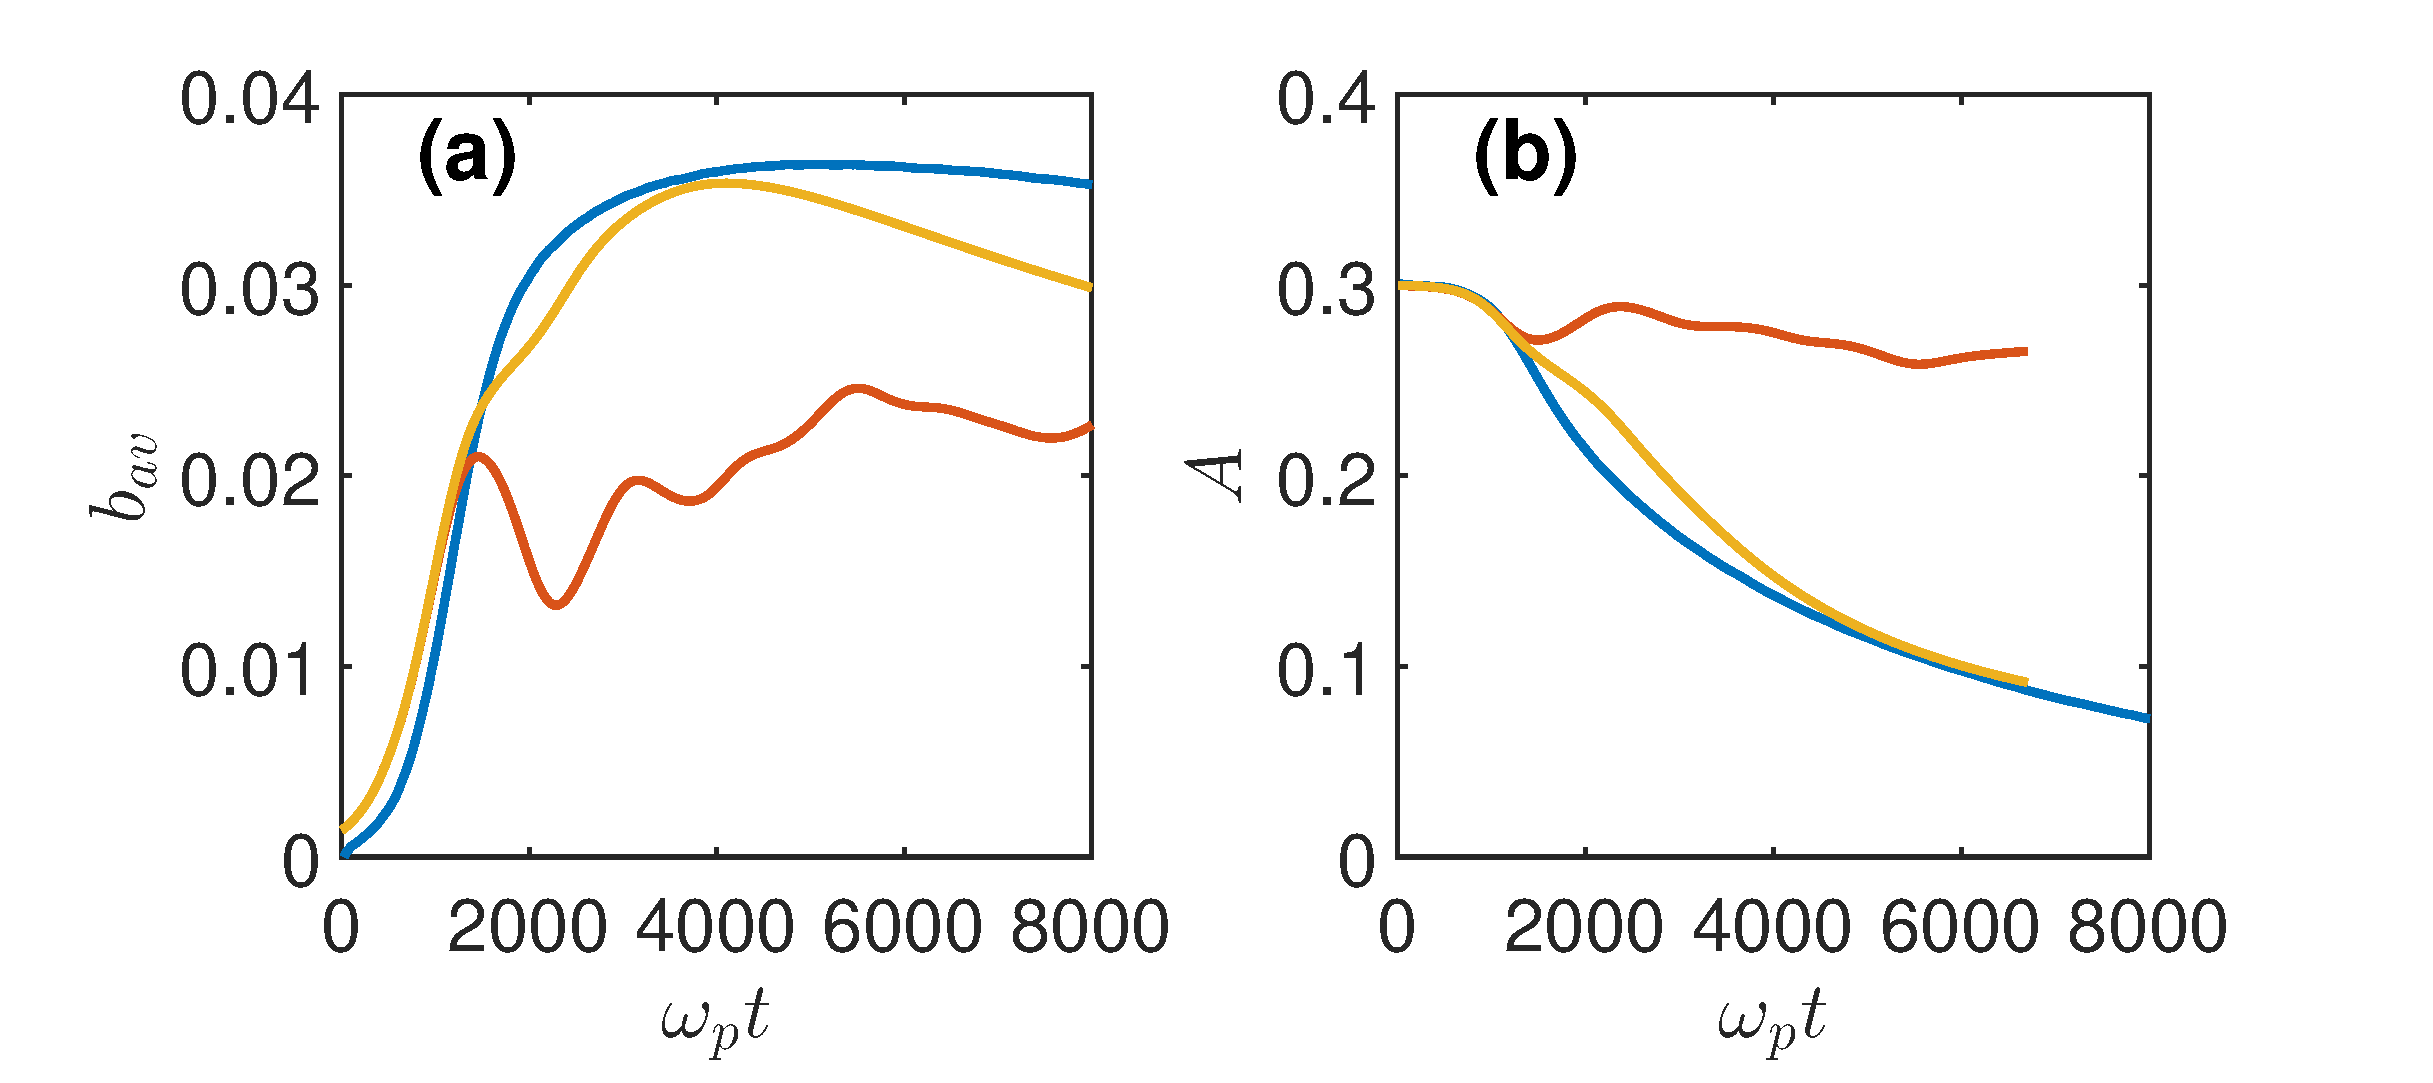
\includegraphics[width=1\linewidth]{part4/aver_medv.eps}
\captionstyle{normal}
\centering
\caption{Эволюция (a) среднеквадратичного магнитного поля $b_{av}$ и (b) параметра анизотропии $A$ в расчете методом частиц в ячейках (синий цвет), квазилинейном расчете (красный цвет) и квазилинейном расчете с добавлением аномальных столкновений (желтый цвет). Внешнее магнитное поле $b_{ext}=0.05$. Начальная анизотропия равна $A_0=0.3$.}
\label{fig:anom_aver}
\end{figure}

Сравнение рис. \ref{fig:anom_spectr}d и рис. \ref{fig:anom_spectr}f иллюстрирует обсуждаемые в разделе \ref{ch:ch4/sec7} расхождения в эволюции динамического спектра магнитоактивной турбулентности вейбелевского типа в квазилинейном подходе и полностью нелинейных расчетах методом частиц в ячейках. 
На значительном временном промежутке добавление аномальных столкновений в квазилинейные расчеты приводит их в соответствие с методом частиц ячейках практически при любых волновых числах за исключением, может быть, наиболее длинноволновой области  $K<0.12$ (ср. рис. \ref{fig:anom_spectr}e и рис. \ref{fig:anom_spectr}f).
Как следует из работы~\cite{Emelyanov2025}, а также из полученных результатов (ср. рис. \ref{fig:anom_spectr}a, \ref{fig:anom_spectr}b и \ref{fig:anom_spectr}c) корректный учет аномальных столкновений играет ключевую роль в правильном определении текущих инкрементов мод на протяжении их нелинейной эволюции.
В длинноволновой области при $K<0.12$ наблюдаемые значения инкрементов оказываются занижены относительно расчетов методом частиц в ячейках, так что когда моды этой области дорастают до значимых значений амплитуды магнитного поля $|b_K|$, корректность квазилинейного описани вновь нарушается.

\begin{figure}[h!]
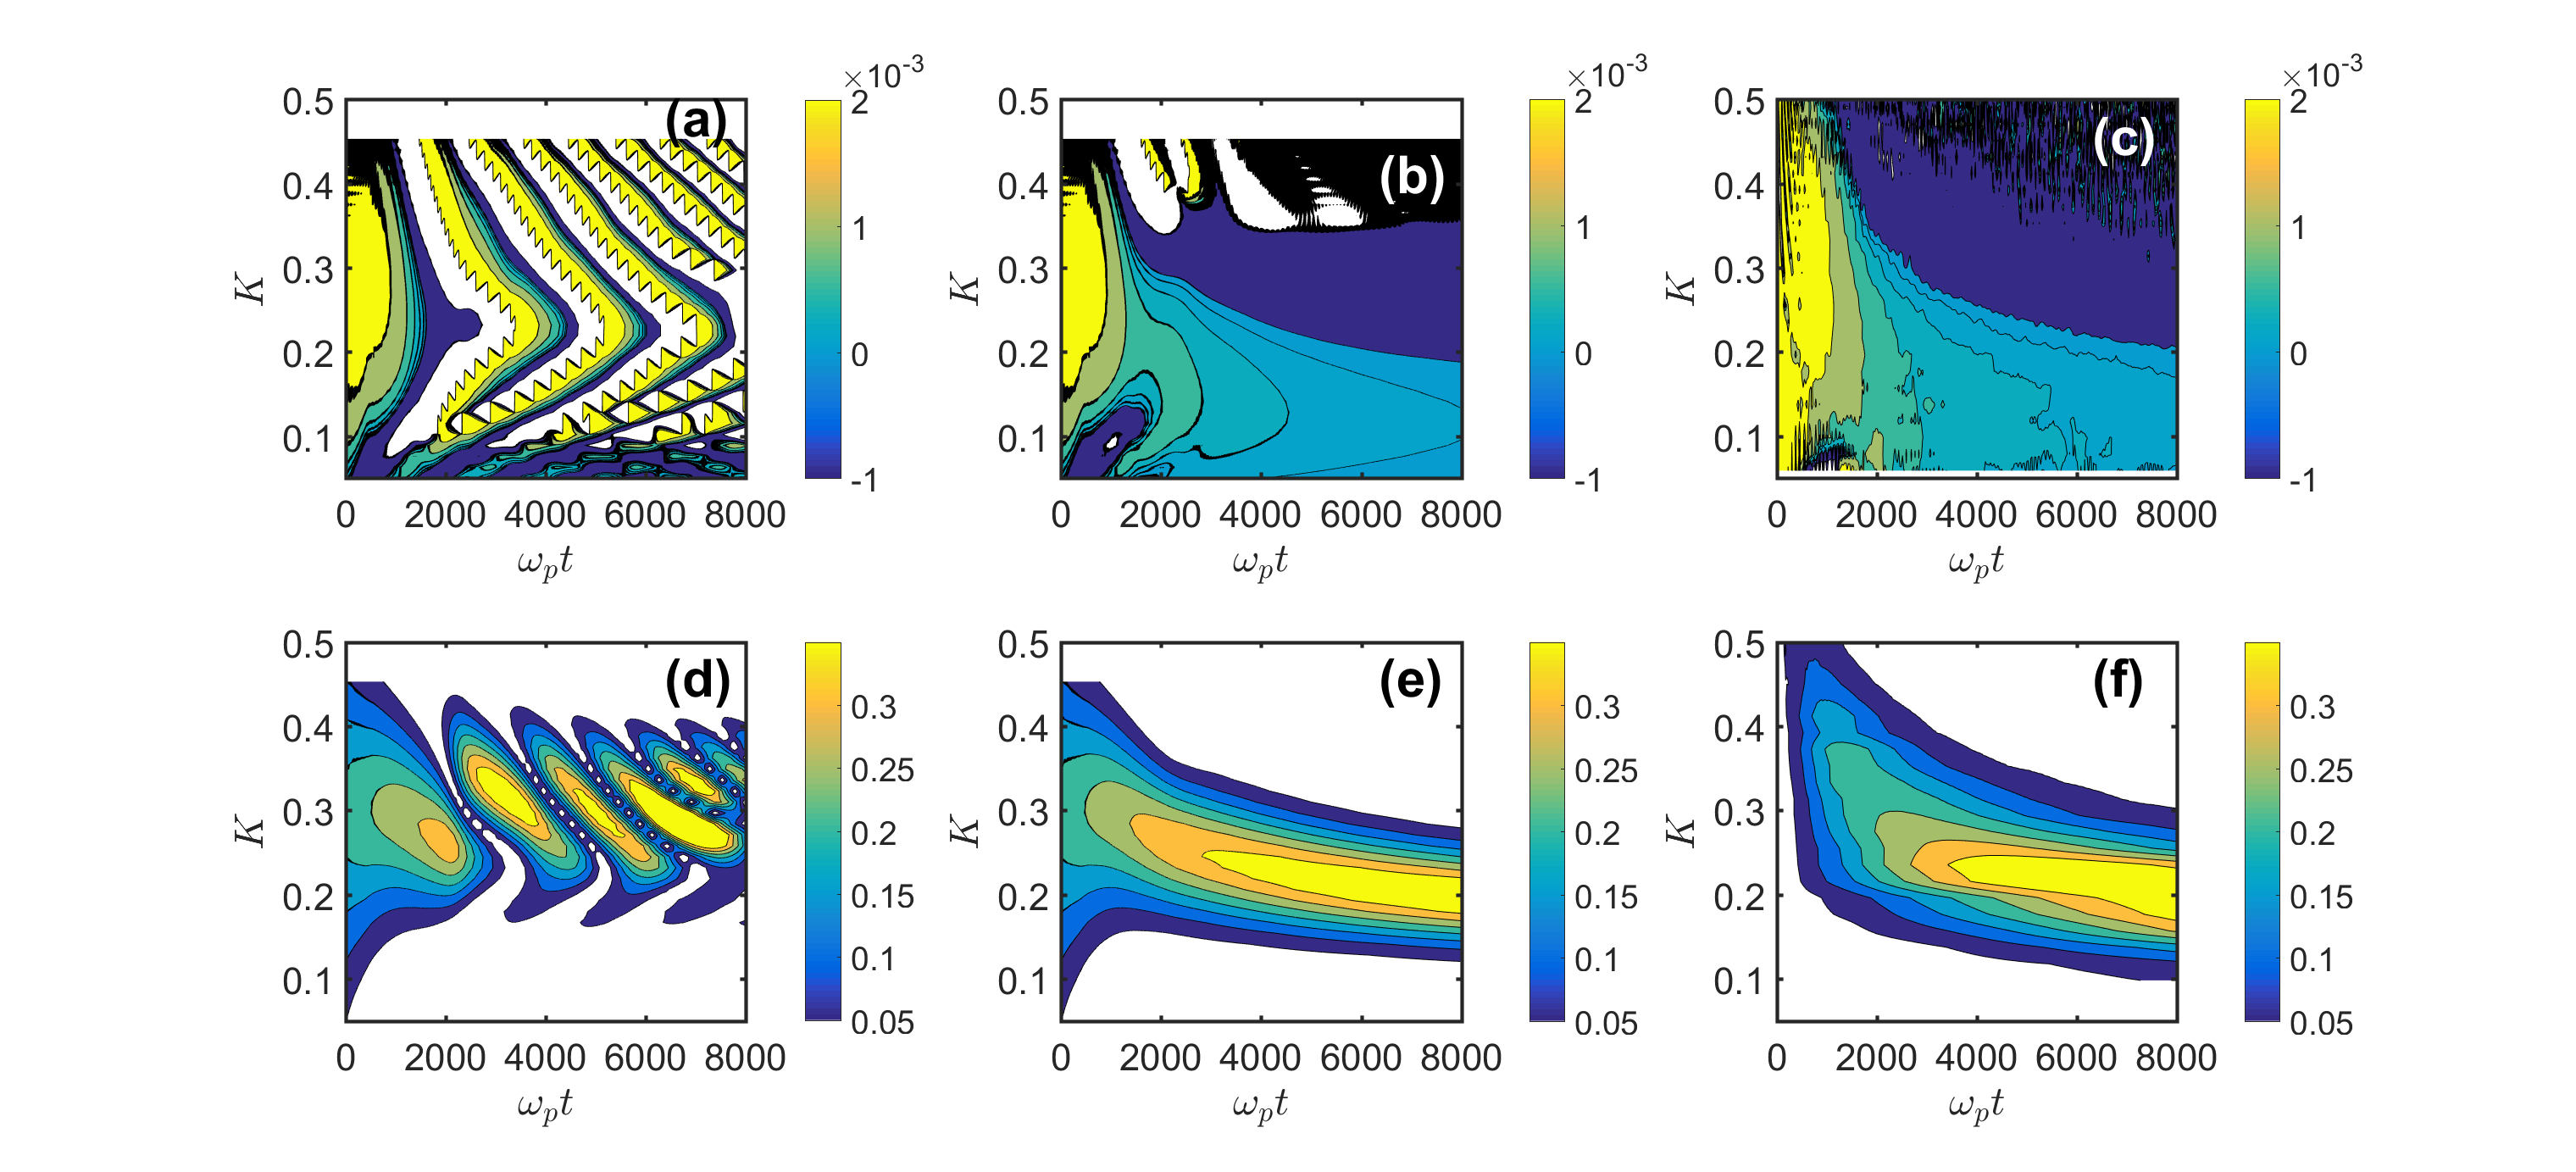
\includegraphics[width=1\linewidth]{part4/spectr_medv.eps}
\captionstyle{normal}
\centering
\caption{Линии уровня текущих инкрементов $\gamma_K(\tau)$ усредненных по аксиальному углу мод магнитного поля $|b_K|$, найденные в двумерных аксиально симметричных расчетах (a) в рамках квазилинейного подхода, (b) в рамках квазилинейного подхода с аномальными столкновениями, (c) методом частиц в ячейках. 
Линии уровня десятичного логарифма амплитуд усредненных по аксиальному углу мод магнитного поля $|b_K|$ спектра турбулентности, найденные в тех же расчетах (d) в рамках квазилинейного подхода, (e) в рамках квазилинейного подхода с аномальными столкновениями, (f) методом частиц в ячейках. 
Внешнее магнитное поле $b_{ext}=0.05$. Начальная анизотропия равна $A_0=0.3$.}
\label{fig:anom_spectr}
\end{figure}

Ввод аномальных столкновений в квазилинейную теорию способствуют значительному расширению применимости последней к плазменным средам, в которых при развитии квазимагнитостатической турбулентности ключевую роль играет не только квазилинейное, но и прямое нелинейное межмодовое взаимодействие. 
В частности, при умеренном магнитном поле, при котором область линейной неустойчивости значительно обузилась, но поперечные моды остаются неустойчивыми, в акисальносимммтриечной задаче удается корректно описать спектральную эволюцию на временах, многократно превосходящих момент насыщения экспоненциального роста.